\chapter{Technologies used for the realisation of the DO}

The following chapter describes the technologies that were used for the development of the DO. Some of the described technologies are not used in final version of the project. However, they are mentioned here, because they were either used at some stage of the project or they were considered as potentially useful and compared between each other.

\section{White Rabbit} \label{section:WR}
    %Ask Maciek if the IEEE 1588-2008 specification is accessible.
    The White Rabbit is a deterministic network based on the Synchronous Gigabit Ethernet. It extends the Precision
    Time Protocol with the precise knowledge of the link delay model and the clock syntonisation over the physical
    layer \cite{wr_master}.
    The WR network consists of two blocks:
    \begin{itemize}
        \item White Rabbit Switch --- it is the main component of the White Rabbit Network. Except for the standard functionalities of an Ethernet switch, it implements the Synchronous Ethernet and the extended PTP in order to distribute the time and the frequency together with the packets of data. It uses redundant network topology to provide reliable communication and a deterministic delivery \cite{wrs}. 
        \item White Rabbit Node --- while the White Rabbit Switches allow to create hierarchical network topology and route the streams of data, the White Rabbit Node is a crucial component for the final user, allowing to integrate the WR technology in custom projects. Implementation of the node is design specific, yet it has to fulfil certain requirements. In order to ease that, the White Rabbit PTP Core was developed. It is an HDL IP-core, containing all the components necessary for the WR integration \cite{ptp_master}.
    
    \end{itemize}
    The topology of WR, presented in Fig. \ref{fig:wr_topology}, is a tree with a System Timing Master at the root. 
    
    \begin{figure}
    	\centerline{\includegraphics[width=0.85\textwidth]{figures/WR_topology.pdf}}
    	\caption{Topology of the WR network}
    	\label{fig:wr_topology}
    \end{figure}
    
    The devices are connected using two types of links:
    \begin{itemize}
        \item up-link ports
        \item down-link ports
    \end{itemize}
    The up-link ports receive the timing information, down-link ports propagate the timing information. WR switches use both types of ports, connecting the branches of the tree.  WR nodes use only the up-link ports, being at the bottom of the tree. 
    
    The System Timing Master receives the clock from an external source, e.g. GPS or an atomic clock, and creates point-to-point connections with devices from the next layer. Each switch can create connections with multiple switches. If the connection with one of the up-link ports is lost, it can seamlessly switch the reference clock without losing the synchronisation.
    
    Two main technologies used in WR are the PTP and the Synchronous Ethernet, described in the following sections.


    \subsection{Precision Time Protocol} \label{subsec:PTP}
        The synchronisation model used in WR is based on the IEEE 1588-2008 PTP (Precision Time Protocol). The PTP synchronises devices in distributed systems, based on the timestamped packets exchange. The principle of the synchronisation is depicted in Fig. \ref{fig:ptp}
        \begin{figure}
        	\centerline{\includegraphics[width=50mm]{figures/ptp.pdf}}
        	\caption{Principle of PTP synchronisation}
        	\label{fig:ptp}
        \end{figure}

        The messages \textit{Sync} and \textit{Delay\_Req} are timestamped with local clocks. Messages \textit{Follow\_Up} and \textit{Delay\_Rep} are used to send the information about the value of the timestamps between the nodes. Having knowledge about the timestamps t\textsubscript{1}, t\textsubscript{2}, t\textsubscript{3} and t\textsubscript{4}, the round trip delay could be calculated using equation \ref{eq:round_trip_delay}. Values t\textsubscript{1} and t\textsubscript{4}, as well as t\textsubscript{2} and t\textsubscript{3} could be subtracted, because they belong to the same clock domain. The results of subtraction are independent of the clock domain, therefore they can also be subtracted in order to obtain the round trip delay. Having the knowledge of the round trip delay, assuming the symmetry of the connection, one way delay is calculated using the equation \ref{eq:one_way_delay}. Knowing the value of the link delay, and the time when the sync message was sent and received, the slave calculates the $offset =  t\textsubscript{2} - t\textsubscript{1} - one\_way\_delay $ between the master's clock and its own clock and uses this value to synchronise to the master \cite{ptp}.
        
        \begin{equation}\label{eq:round_trip_delay}
        round\_trip\_delay = (t_4 - t_1) - (t_3 - t_2)
        \end{equation}
        
        \begin{equation}\label{eq:one_way_delay}
        one\_way\_delay = \frac{round\_trip\_delay}{2}
        \end{equation}
        The accuracy of the clock synchronisation in IEEE-1588-2008 is in the range of microseconds. White Rabbit extends PTP with precise knowledge of the link delay model and takes into account the link asymmetry, obtaining sub-nanosecond synchronisation \cite{wr_spec}.
        
    \subsection{Synchronous Ethernet}
        The precise phase adjustment is possible only when the clocks are syntonised, which means that they are of exactly the same frequency. In the WR network, syntonisation is obtained using the Synchronous Ethernet. 
        The standard Ethernet connection is peer-to-peer, whereas Synchronous Ethernet uses a hierarchical structure, with a System Timing Master on top. Each slave recovers the clock signal from the incoming data stream, using PLLs. The clock is propagated to the next layer of nodes in the data stream \cite{wr_master}.

\section{Spec boards with FPGA Mezzanine Card (FMC) cards}
    The DO requires the use of Analogue to Digital Converter (ADC) boards that support WR. For that purpose two boards are used:
    \begin{itemize}
        \item Simple PCIe FMC carrier (SPEC),
        \item FMC ADC board .
    \end{itemize}
    Both of these boards are open-source and commercially available.
    
    \subsection{SPEC}
        SPEC is a general carrier board. It provides the main components allowing to configure it as the WR node and extend its functionalities using an FMC board \cite{spec_ohwr}:
        
        \begin{itemize}
            \item 4-lane PCIe
            \item Xilinx Spartan6 Field-Programmable Gate Array (FPGA) XC6SLX45T-3FGG484C (in the DO the special version is used: XC6SLX150T)
            \item FMC slot with low pin count (LPC) connector
            \item clocking resources
            \item on board memory
            \item Small Formfactor Pluggable (SFP) cage for fibre-optic transceiver
        \end{itemize}
    
    \subsection{FMC ADC} \label{section:fmc_adc}
        %purpose
        FMC ADC card \cite{fmc_adc_ohwr} is an extension FMC board, which allows digitising the input analogue signal. 
        %implemented functions
        It implements the most standard features of an oscilloscope, that is, the configuration of:
        \begin{itemize}
            \item channels settings:
            \begin{itemize}
                \item range
                \item termination
                \item offset
                \item saturation
            \end{itemize}
            \item trigger settings:
            \begin{itemize}
                \item polarity
                \item delay
                \item threshold (in case of the internal trigger)
            \end{itemize}
            \item acquisition settings:
            \begin{itemize}
                \item pre-samples
                \item post-samples
                \item number of shots
                \item under-sampling
            \end{itemize}
        \end{itemize}
        
        The design of the digitiser consists of 4 layers:
        \begin{itemize}
            \item hardware
            \item gateware
            \item software:
            \begin{itemize}
                \item driver
                \item library
            \end{itemize}
        \end{itemize}
        
        \subsubsection{hardware}
            %what it contains
            The FMC board contains an LTC2174 \cite{datasheet:LTC2174} chip that includes four 14 bits, 100~MS ADCs in one package. It includes 5 LEMO connectors: 4 for input signals and 1 for the external trigger. The impedance of each input is software selectable: 50~$\Omega$/1M~$\Omega$. It contains amplifiers for selecting the input range as well as 16-bit Digital to Analog Converters (DAC) to apply a DC offset to an input signal. It uses the FMC connector to communicate with the SPEC FPGA.
        
        \subsubsection{gateware}
            The FPGA of the carrier board has direct access to the hardware of the board. It is responsible for the low-level configuration of the board features.
            
            \begin{figure}
            	\centerline{\includegraphics[width=0.8\textwidth]{figures/acq_fsm.pdf}}
            	\caption{Finite state machine of the acquisition}
            	\label{fig:acq_fsm}
            \end{figure}
            
            For the purpose of data acquisition, it implements the finite state machine, presented in Fig. \ref{fig:acq_fsm}. At start-up, the finite state machine is in IDLE state. After receiving the signal to start the acquisition, it starts acquiring data, which it writes to the memory using the Direct Memory Access (DMA), and waits for a trigger. After receiving the trigger it acquires the number of post-samples specified by the user. The acquisition is repeated until obtaining the requested number of acquisitions. After that, it returns the obtained data, enters the IDLE state and waits for the signal to start another acquisition \cite{fmc_adc_gateware_guide}. 
            The data written to the memory contains the samples from each channel and the information if the current sample is aligned with the trigger. The data is passed through the timestamping core, that allows determining the time of the trigger.
        
        \subsubsection{software}
            The FPGA resources are accessed by the ADC library, which makes use of the driver. The library provides a generic API for accessing the digitiser boards. It allows to:
            \begin{itemize}
                \item Configure the ADC parameters.
                \item Start the acquisition.
                \item Access the data, together with the information about the trigger and the timestamp.
            \end{itemize}

        
\section{White Rabbit Trigger Distribution} \label{section:WRTD}
    The key element of the DO is White Rabbit Trigger Distribution. It uses WR for clock synchronisation and exchanging data.
    %what is the goal
    \subsection{Purpose of WRTD} \label{subsec:purpose_of_wrtd}
        The purpose of WRTD is the ability to trigger the devices at the specified time. Depending on the application the requirements could be the following:
        \begin{itemize}
            \item Trigger the devices at exactly the same time.
            \item Trigger the devices with well specified delay between the triggers. 
        \end{itemize}
        Depending on the configuration, the WRTD can fulfil both of the requirements. 
    
    \subsection{Basic block of WRTD} \label{subsec:WRTD_block}
        %the building block
        The WRTD network is constructed of the basic building blocks, which share the same time reference determined by the 125~MHz clock of WR. The schematic of the WRTD block is depicted in Fig. \ref{fig:wrtd_block}.
        \begin{figure}
        	\centerline{\includegraphics[width=100mm]{figures/wrtd_block.pdf}}
        	\caption{Basic building block of the WRTD network}
        	\label{fig:wrtd_block}
        \end{figure}
        %local connections
        \textit{Local in} and \textit{Local out} are connections with devices to which there is a direct physical access. The devices that could be potentially connected are the following:
        \begin{itemize}
            \item Input devices:
            \begin{itemize}
                \item WRTD enabled ADC, generating the trigger when the measured value crosses the threshold voltage.
                \item Time to Digital Converter --- device that generates the timestamp at the time specified by the edge of the incoming pulse signal.
            \end{itemize}
            \item Output devices:
            \begin{itemize}
                \item WRTD enabled ADC, triggering on the time determined by the timestamp.
                \item Fine Delay --- device that generates the pulse at the time specified by the timestamp.
            \end{itemize}
        \end{itemize}
        %remote connections
        \textit{Remote in} and \textit{Remote out} are the connections with other WRTD blocks. Each output message from the connection that is not specified as local is sent over the network and could be used to trigger the devices connected to any of the other WRTD blocks. Each block could receive or discard the message depending on the rules set by the user, which will be described in the next sections.

    %API
    \subsection{WRTD API}
        The behaviour of the network is specified using the WRTD API. The structure and the functions available in the API were written in a way to be as compliant with LXI as possible. The available functions are listed in Tab. \ref{tab:wrtd_api}.
        
        The library contains the following types of functions:
        \begin{itemize}
            \item General --- initialisation, resetting and closing of the library as well as monitoring the internal state of the library
            \item Error handling
            \item Logs management
            \item Rules management --- the rules are responsible for interconnection of the blocks
            \item Alarms management --- alarms define at what time the event should be generated
            \item Attributes setters --- attributes modify the behaviour of the rules and the alarms
            \item Attributes getters
        \end{itemize}
        
        \begin{table}
\centering
\caption{List of the functions from the WRTD API}
\begin{tabular}{cc}
Type of function & Name of the function \\
\hline
\hline
\multirow{5}{*}{General} 
& wrtd\_init \\                                                                
& wrtd\_close \\                                                                  
& wrtd\_reset \\ 
& wrtd\_get\_sys\_time \\                                                      
& wrtd\_reset\_rule\_stats \\   
\hline
\multirow{2}{*}{Error handling} 
& wrtd\_get\_error \\                                                             
& wrtd\_error\_message \\  
\hline
\multirow{2}{*}{Logs management} 
& wrtd\_log\_read \\                                                           
& wrtd\_clear\_log \\ 
\hline
\multirow{5}{*}{Rules management} 
& wrtd\_add\_rule \\                                                           
& wrtd\_disable\_all\_rules \\                                                    
& wrtd\_remove\_rule \\                                                           
& wrtd\_remove\_all\_rules \\                                                     
& wrtd\_get\_rule\_id \\  
\hline
\multirow{5}{*}{Alarms management} 
& wrtd\_add\_alarm \\                                                          
& wrtd\_disable\_all\_alarms \\                                                
& wrtd\_remove\_alarm \\                                                       
& wrtd\_remove\_all\_alarms \\                                                 
& wrtd\_get\_alarm\_id \\ 
\hline
\multirow{5}{*}{Attributes setters} 
& wrtd\_set\_attr\_int32 \\                                                    
& wrtd\_set\_attr\_int64 \\                                                    
& wrtd\_set\_attr\_bool \\                                                     
& wrtd\_set\_attr\_tstamp \\                                                   
& wrtd\_set\_attr\_string \\   
\hline
\multirow{5}{*}{Attributes getters} 
& wrtd\_get\_attr\_int32 \\                                                       
& wrtd\_get\_attr\_int64 \\                                                    
& wrtd\_get\_attr\_bool \\                                                        
& wrtd\_get\_attr\_tstamp \\                                                      
& wrtd\_get\_attr\_string \\   
\end{tabular}
\label{tab:wrtd_api}
\end{table}
        
    \subsection{Example of usage}
        In order to explain how the library works, the example of the library configuration is presented. The examples fulfil the requirements specified in section \ref{subsec:purpose_of_wrtd}.
        
        \subsubsection{Fixed delay} \label{subsec:WRTD_fixed_delay}
            In order to be able to trigger one device with another with a fixed, well known delay, appropriate rules have to be set and configured. Each rule has 4 attributes:
            \begin{itemize}
                \item Source --- determines which event/device is the source of the trigger.
                \item Destination --- determines which device/connection should be triggered.
                \item Delay --- determines the amount of time that should be added to the timestamp.
                \item Enable --- determines if the given rule is enabled.
            \end{itemize}
            In order to connect two remote devices, two rules have to be established, with an example configuration presented in Tab. \ref{tab:wrtd_example}.
            
            \begin{table}
            \centering
            \caption{Example configuration to connect two devices using WRTD}
            \begin{tabular}{ccc}
            Attribute & Triggering device --- ADC1 & Triggered device --- ADC2 \\
            \hline
            Source & LC-I0 & LAN1 \\
            Destination & LAN1 & LC-O0 \\
            Delay & 500~ns & 0 \\
            Enable & 1 & 1 \\
            \end{tabular}
            \label{tab:wrtd_example}
            \end{table}
            
            The schematic of this connection are presented in Fig. \ref{fig:wrtd_connection}.
            
            \begin{figure}
            	\centerline{\includegraphics[width=\textwidth]{figures/wrtd_connection.pdf}}
            	\caption{Example of connectivity of two devices using WRTD}
            	\label{fig:wrtd_connection}
            \end{figure}
            
            An example code for the configuration of the rules for distribution and reception of the WRTD triggers are presented in Lis. \ref{cap:trig_dist} and Lis. \ref{cap:trig_rec} respectively.
            
            \input{listings/wrtd_examples.tex}
            
            LC-I0 means local input connection, LC-O0 means local output connection. With such a configuration, the triggering device will send a timestamp to the remote connection called LAN1, when there will be some event on its local connection. The value of the timestamp will be equal to the time when the event was produced, plus the time specified as the delay, in this case 500~ns. The triggered device will produce an event on its local connection at the time specified by the timestamp received on the LAN1 remote connection. In order to trigger the second device at the required time, the user has to make sure that the value of the delay is bigger than the worst-case delay of the network. The worst-case delay can be calculated based on the length of the cables that connect the devices in the WR Network and the delays of the particular elements of the network. 
        
        \subsubsection{Triggering at the same time}
            In order to trigger devices at a specified time, WRTD provides the functionality of alarms. The user can add an alarm that will trigger the devices at the specified time. Because of the common time reference, if various ADCs have the same value of the alarm, they will trigger at the same time.
            
    \subsection{implementation}
        In order to configure the WRTD, the FPGA resources have to be accessed. The access is provided by means of the mockturtle framework. 
        
        %mockturtle
        The essential components of this framework are the soft Central Processing Units (CPU) cores implemented in the FPGA. Each of the cores can run a different C application. In order for the soft CPU cores to communicate with the host machine, the mockturtle framework implements the mechanism of message queues. 
        
        WRTD implements a firmware for the mockturtle cores, in order to allow an access to the required FPGA cores \cite{mockturtle_ohwr}. The WRTD API is built on top of this firmware and hides the implementation details. The code that makes use of the API is run on the host machine. The user of the WRTD does not have to know anything about the mockturtle nor the firmware.
        
\section{Communication}
    In distributed systems, one of the main issues that have to be solved is to establish communication between the nodes. The problem is split into three parts:
    \begin{itemize}
        \item enumeration of the devices
        \item communication using Remote Procedure Calls (RPC)
        \item data transmission
    \end{itemize}
    The available technologies that may be used to solve the issues are presented in the following sections:
    
    \subsection{Enumeration of the devices} \label{subsec:zeroconf}
        %Problem description
        In distributed systems, one of the problems that have to be solved is how to detect available devices. 
        %First solution
        The common solution is to have a central unit, to which each new device connects when it is added to the network. For this, the devices have to be properly configured to know what the address of this central unit is. 
        
        %Second solution
        In order to avoid the necessity of manual configuration, many of the laboratory equipment use zeroconf networking. There exist various libraries for this purpose. In DO Python-Zeroconf~\cite{zeroconf} is used because it is the most common library in Python. 
        
        In Python-Zeroconf the server broadcasts the necessary information to create a connection: in the most basic case its IP address and the port on which it is listening. The device that appears in the network receives that information and automatically connects. The restriction of that technology is that it is limited to local networks.

    \subsection{Remote Procedure Call} \label{subsec:chap3:communication:rpc}
         RPCs allow executing the functions on remote clients. RPC eases the integration of applications, allowing invoking remote procedures as if they were local. However, it is important to distinguish if the call is local or remote because the RPC could be orders of magnitude slower than the local call, as well as less reliable. 
        
        It is typically implemented using a request-response messaging pattern. Applications that want to expose some functionalities provide a set of functions that can be executed, which is known by both the server and the client. The function that is executed on the server depends on the request of the client, which receives the result of the operation in the response.
        
        There is a great variety of available RPC libraries, among which the most common are:
        \begin{itemize}
            \item XML-RPC --- it is available in The Python Standard Library. It uses Extensible Markup Language (XML) for data transport, therefore it is not very efficient if a great amount of data should be sent between the client and the server.
            \item gRPC --- it is the RPC developed by Google. It is very efficient, yet more complicated to start using than the other libraries. It uses google protocol buffers for serialisation of data.
            \item RPyC --- it is a library mainly optimised for ease of use and "seamless RPC". It allows easy integration of applications, yet for an inexperienced user, it is not necessarily the best choice because it creates an illusion that there is no difference between the local and the remote call.
            \item own implementation --- RPC could be easily implemented using request-reply pattern with any type of transport, e.g. raw TCP or ZeroMQ. In some cases, this could be the best option, since the user can implement all the required features, without depending on the external library and without any overhead in the development time.
            %Probably in the implementation chapter write about the fact, explain that the RPC should not be complicated nor nested, because they could lead to blocking of the program, especially that it is more difficult to debug the problem if it is on two different machines. 
            %in the implementation chapter write what are the requirements, what did I try, how I did the final decision
        \end{itemize}
        For reasons presented in section \ref{section:rpc_selection}, own implementation of the RPC was chosen. After doing a series of measurements, presented in section \ref{section:data_transport_opt}, ZeroMQ library was chosen as a data transport.
    
    \subsection{Data transmission} \label{subsec:ZeroMQ}
        For data transmission, the ZeroMQ library was chosen. ZeroMQ is an open-source asynchronous messaging library. It is optimised mainly for high performance and low latency. It aims at large distributed systems, where the problem of scalability becomes an issue. The API is designed to resemble the Berkeley sockets. It implements various features that the developer would have to handle himself using the raw TCP. The key features are the following:
        \begin{itemize}
            \item The input/output operations are handled in background threads, using lock-free data structures, which allows scaling the applications easily. 
            \item It automatically queues the messages and provides the features to deal with high water marks. 
            \item The format of the messages is not imposed. It allows using the built-in serialiser, as well as to use any kind of the product on top.
            \item It automatically reconnects in case of lost connection and allows connection of the nodes in an arbitrary order.
            \item It allows establishing communication between the applications using arbitrary transports: TCP, inter-process or in-process.
        \end{itemize}
        ZeroMQ supports many messaging patterns, for which the library provides various types of sockets:
        \begin{itemize}
            \item REQ/REP --- they are meant for a simple synchronous request-reply pattern, where each request expects one reply.
            \item DEALER/ROUTER --- they extend the request-reply pattern allowing for an asynchronous operation.
            \item PUSH/PULL --- they are meant for distributing large amounts of data, in one direction.
            \item PUB/SUB --- they are used to distribute data in nodes arranged in the pipeline.
            \item RADIO/DISH --- they are used to distribute data from a single publisher to multiple subscribers
            \item CLIENT/SERVER --- they are used to create standard client-server applications, where the client initiates the conversation and the server can talk to one or multiple clients.
        \end{itemize}
        More advanced scenarios could be implemented using combinations of the described sockets \cite{zeromq_guide}.
        
    
    %In the optimisation and/or implementation : Do the measurements, compare it, chose the best solution, don't forget to take into account the simplicity of the solution, not only the efficiency
    \subsection{Serialisation} \label{subsec:serialisation}
        In distributed systems, the data sent between the nodes has to be converted into some format that is understandable by all the nodes. In the following section various data formats and serialisation libraries are presented: 
        
        \subsubsection{Pickle}
            Pickle is a Python native library that implements binary protocols for serialisation and deserialisation of data. It is intended only for Python. The obvious consequences are that it is not possible to share data with code that is written in a different language, yet it is well optimised for Python. The major difference between pickle and generic serialisation libraries is that it keeps track of the objects that were already serialised, avoiding serialising the same object twice. Since it is a binary protocol, it is not human readable \cite{pickle}.
        
        \subsubsection{JavaScript Object Notation (JSON)}
            JSON is a data-interchange format that is designed to be easy to read and write for humans, as well as easy to parse and generate for machines. The data is represented in text format. The JSON is language-independent \cite{json}.
        
        \subsubsection{Protocol Buffers}
            Protocol Buffers are a mechanism for serialising data. They allow users to define the data structures in .proto files, then, using the protocol buffer compiler, they generate the data access classes, which can be included in the code. Protocol Buffers separate the data representation and serialisation, making it both human readable as well as efficient. They are language-independent \cite{protobuf}.

\section{Qt} \label{section:qt}
    Qt is an open-source toolkit for creating Graphical User Interfaces. It provides an environment for quick development of applications called QtCreator. It uses an event-driven programming model for interaction with the user. It allows easy integration with other libraries, as well as the development of critical elements of the application without using Qt constructs. It is written in C++, but provides bindings for many different languages, including Python. 
